\section{Electron Matter Interactions}
To understand the working principle of a \ac{sem}, it is necessary to consider the
interaction between electrons and solid matter.
For that, one observes the path of an electron which is emitted directly from the cathode
and head to the sample. Those electrons are called \textit{\ac{pe}}.
After arriving at the surface, the electrons undergo elastic and inelastic scattering.
Due to complex interactions between \ac{pe} and the atoms
inside the sample, multiple interaction products are generated, which can
be classified into different categories.
The categories, that are relevant for conducing the experiment are the
following:
\begin{itemize}
	\item Secondary electrons
	\item Backscattered electrons
	\item X-Ray emission
\end{itemize}
After arriving at the surface, the electrons spread due to
small-angle scattering in a pear shaped area around the collision point.
Different interactions are located at different spatial regions.
This is visualized in \cref{fig:birne}.
The higher the atomic number, the stronger is the scattering of the
electrons.
\subsection{Secondary Electrons}
\ac{pe} collide with the bounded electrons and ionize the
corresponding atoms.
Those now free electrons from the top layer can diffuse out of the
material and are called \ac{se}.
Due to the high energy loss during ionization, \ac{se}
have a low kinetic energy compared to \ac{pe}.
The energy distribution is shown in \cref{fig:electrons}.
To quantify the relation between \ac{pe} and \ac{se}, one
uses the electron yield $\delta_\mathrm{SE} = \text{\# SE} / \text{\# PE}$.
In the typical case of \ac{pe} with energies between
\qtyrange{10}{25}{\kilo\electronvolt}, $\delta_\text{SE}$ is far below one.
It is possible to get a topographic contrast from \ac{pe}.
The electron yield is strongly dependent on the angle of incidence of
the surface with $\delta_\mathrm{SE} \simeq \cos(\theta)$.
If there is a change in height, there must also be a change of the
incidence angle $\theta$ which alters the image.
Note, that only height changes and not the absolute height defines the
topography contrast.
Due to the fact, that the absorption length for secondary electrons is
only a couple nanometers thin, this method delivers precise information
about a local structure.
\begin{figure}[H]
	\centering
	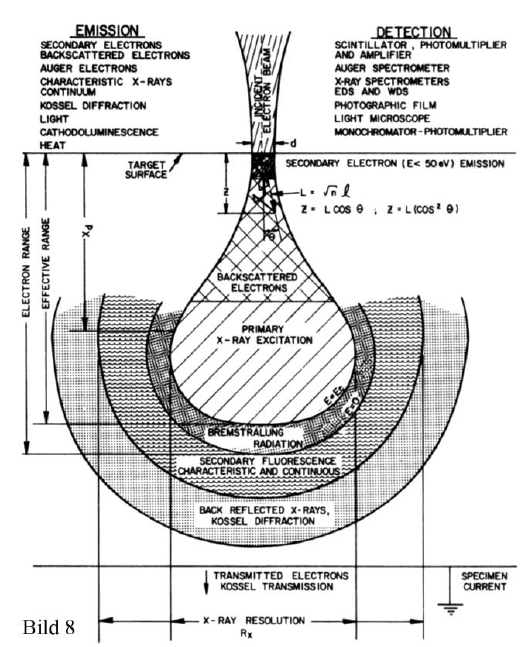
\includegraphics[width=0.95\linewidth]{../assets/birne.png}
	\caption{Interaction area of electrons. \imcite{rem_script}}
	\label{fig:birne}
\end{figure}
\ac{se} are caught by the detector and converted into
an electrical signal.
The scanning electron microscope uses a light-sensitive photo multiplier
with a scintillator disc and a metal grid for collecting electrons.
The metal grid and the scintillator disk can be biased to filter
electrons with different energies.
For \ac{se}, the metal grid is positively charged to attract electrons
from a larger spatial region.
After the electrons collide with the scintillator, the material emits
light, which can be detected by the photo multiplier.
The more electrons collide with the scintillator, the higher is the
intensity of the emitted light and the stronger is the
electrical signal which leads to a brighter pixel on the image.

Not only the surface topography can affect the electron yield but also
the electrical surface potentials.
\begin{figure}[H]
	\centering
	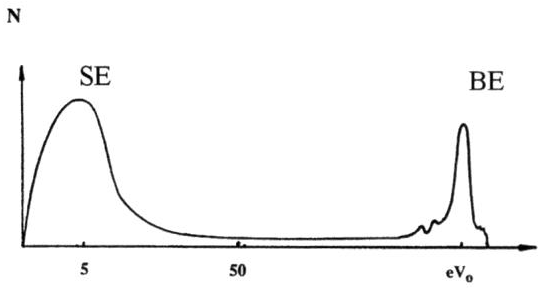
\includegraphics[width=0.95\linewidth]{../assets/elektronen.png}
	\caption{Electron yield as a function of energy. \imcite{rem_script}}
	\label{fig:electrons}
\end{figure}

\subsection{Backscattered Electrons}
A large proportion of \ac{pe} won't ionize the material but
rather be reflected or backscattered by the nuclei of the sample.
Due to the heavy nucleus, the electrons will primarily change their
direction.
These electrons are called \ac{be}. In a physical sense, \ac{be} can't be
distinguished from \ac{se}, but their kinetic energy is much higher
which provides a good indicator.
This leads to the definition that electrons with energies in the order
of magnitude of $\mathrm{e} V_0$, where $\mathrm{e}$ is the elementary
charge and $V_0$ the potential difference of the cathode, are
categorized as \ac{be}.

The electron yield for backscattered electrons is very dependent on
the atomic number $Z$ with $\delta_\text{BS} = \# BS / \# PE
	\propto \sqrt{Z}$.
Because of this dependency and the fact, that \ac{be}
contrast is less affected by surface layers and local surface fields,
they offer a reliable
method to detect material contrast.
This is visualized in \cref{fig:material_contrast}.

To detect \ac{be}, one can use a solid-state p-n
junctions with multiple sectors.
Those detectors are reverse biased to establish an electric field which
can collect and count the arriving electrons.
A stronger signal corresponds to a higher number of collected electrons.
\begin{figure}[H]
	\centering
	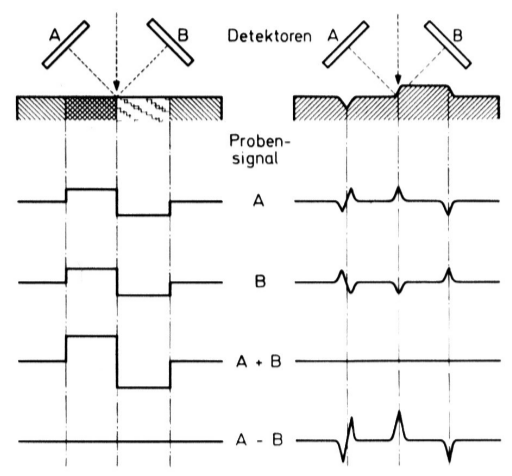
\includegraphics[width=0.95\linewidth]{../assets/material.png}
	\caption{Material contrast (left) and topographical contrast (right) detection.
		\imcite{rem_script}}
	\label{fig:material_contrast}
\end{figure}

\subsection{X-ray Emission}
The X-ray spectrumlconsists of two parts.
The first part consists of bremsstrahlung, which is generated during the
deceleration of the electrons.
This type of radiation is, due to it's origin, observable in every X-ray
emission experiment and cannot be used to identify materials.

For that, there exists the second part, which is called characteristic
radiation.
During ionization, electrons from energetically higher states relax
into a more favorable states.
The resulting energy differnce generates an X-ray photon.
Due to the  discrete energies of the electron states,
the resulting energy-intensity spectra will contain sharp, well-defined
peaks, which are characteristic for every material.
The energy transitions $K_{\mathrm{\alpha}_{1}}$ and
$K_{\mathrm{\alpha}_{2}}$ are primarely observed.

To analyse X-ray radiation, one can conduct an energy dispersive
spectrometer experiment.
A cooled silicium diode detector is driven reverse biased to create an
electric field.
If an X-ray photon enters the material, it will create electron-hole-pairs
which can be separated and counted.
The higher the number of electrons, the higher the energy of the X-ray
photon.
By analyzing the positions of the peaks in the spectrum, qualitative
conclusings about the compositions can be drawn.
Through the corresponding intensity, quantitiative conclusions are also
possible.
